\documentclass{standalone}
\usepackage{tikz}
\usepackage{verbatim}
\usetikzlibrary{positioning}
\begin{document}
\pagestyle{empty}
  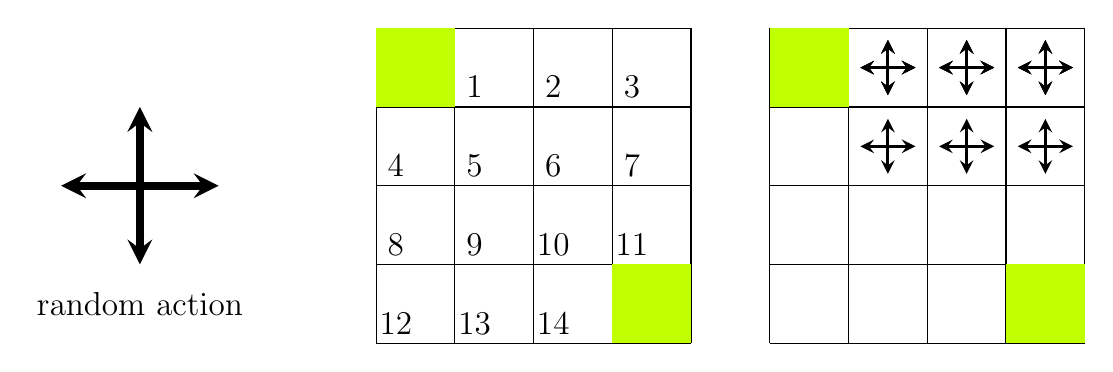
\begin{tikzpicture}
    \draw[stealth-stealth, line width=1 mm] (-4, 2) -- (-2, 2);
    \draw[stealth-stealth, line width=1 mm] (-3, 1) -- (-3, 3);
    \node at (-3, 0.5) {\large random action};
    \draw[step=1.0,black,thin] (0,0) grid (4, 4);
    \fill[lime] (0, 3) rectangle (1,4);
    \fill[lime] (3, 0) rectangle (4,1);
    % Top row.
    \node at (1.25, 3.25) {\large 1};
    \node at (2.25, 3.25) {\large 2};
    \node at (3.25, 3.25) {\large 3};
    % Second frop top row.
    \node at (0.25, 2.25) {\large 4};
    \node at (1.25, 2.25) {\large 5};
    \node at (2.25, 2.25) {\large 6};
    \node at (3.25, 2.25) {\large 7};
    % Second from bottom row.
    \node at (0.25, 1.25) {\large 8};
    \node at (1.25, 1.25) {\large 9};
    \node at (2.25, 1.25) {\large 10};
    \node at (3.25, 1.25) {\large 11};
    % Bottom row.
    \node at (0.25, 0.25) {\large 12};
    \node at (1.25, 0.25) {\large 13};
    \node at (2.25, 0.25) {\large 14};
    
    \draw[step=1.0,black,thin] (5,0) grid (9, 4);
    \fill[lime] (5, 3) rectangle (6,4);
    \fill[lime] (8, 0) rectangle (9,1);
    % Top row.
    \draw[stealth-stealth, line width=0.4mm] (6.15, 3.5) -- (6.85, 3.5);
    \draw[stealth-stealth, line width=0.4mm] (6.5, 3.15) -- (6.5, 3.85);
    \draw[stealth-stealth, line width=0.4mm] (7.15, 3.5) -- (7.85, 3.5);
    \draw[stealth-stealth, line width=0.4mm] (7.5, 3.15) -- (7.5, 3.85);
    \draw[stealth-stealth, line width=0.4mm] (8.15, 3.5) -- (8.85, 3.5);
    \draw[stealth-stealth, line width=0.4mm] (8.5, 3.15) -- (8.5, 3.85);
    % Second from top row.
    \draw[stealth-stealth, line width=0.4mm] (6.15, 2.5) -- (6.85, 2.5);
    \draw[stealth-stealth, line width=0.4mm] (6.5, 2.15) -- (6.5, 2.85);
    \draw[stealth-stealth, line width=0.4mm] (7.15, 2.5) -- (7.85, 2.5);
    \draw[stealth-stealth, line width=0.4mm] (7.5, 2.15) -- (7.5, 2.85);
    \draw[stealth-stealth, line width=0.4mm] (8.15, 2.5) -- (8.85, 2.5);
    \draw[stealth-stealth, line width=0.4mm] (8.5, 2.15) -- (8.5, 2.85);
    % Second from bottom row.
    \draw[stealth-stealth, line width=0.4mm] (6.15, 3.5) -- (6.85, 3.5);
    \draw[stealth-stealth, line width=0.4mm] (6.5, 3.15) -- (6.5, 3.85);
    \draw[stealth-stealth, line width=0.4mm] (7.15, 3.5) -- (7.85, 3.5);
    \draw[stealth-stealth, line width=0.4mm] (7.5, 3.15) -- (7.5, 3.85);
    \draw[stealth-stealth, line width=0.4mm] (8.15, 3.5) -- (8.85, 3.5);
    \draw[stealth-stealth, line width=0.4mm] (8.5, 3.15) -- (8.5, 3.85);
    % Bottom row.
    \draw[stealth-stealth, line width=0.4mm] (6.15, 3.5) -- (6.85, 3.5);
    \draw[stealth-stealth, line width=0.4mm] (6.5, 3.15) -- (6.5, 3.85);
    \draw[stealth-stealth, line width=0.4mm] (7.15, 3.5) -- (7.85, 3.5);
    \draw[stealth-stealth, line width=0.4mm] (7.5, 3.15) -- (7.5, 3.85);
    \draw[stealth-stealth, line width=0.4mm] (8.15, 3.5) -- (8.85, 3.5);
    \draw[stealth-stealth, line width=0.4mm] (8.5, 3.15) -- (8.5, 3.85);
  \end{tikzpicture}
\end{document}